\documentclass{ximera}

\input{../../preamble.tex}

\title{Assembly Line}

\begin{document}

\begin{abstract}
composition
\end{abstract}
\maketitle





Mathematics is a language. It is a tool we use to describe structure. Functions are a part of this language. We use functions to describe relationships, associations, and connections.

We also use functions to describe processes.

We use functions to describe an ordered application of actions. We might see this as step-by-step instructions, an algorithm, or an assembly line.



\textbf{For example,} in a bottling plant the cap is not attached before the beer is poured into the bottle. Beer first, then cap.


\textbf{For example,} the tires are not screwed to the chassi of the car before it is dipped into the rust prevention tank.


\textbf{For example,} Flour, sugar, oil, and eggs are mixed together before baking.





\begin{definition} \textbf{\textcolor{green!50!black}{Composition}}


Let $F$ and $G$ be two functions.

The \textbf{composition of $F$ and $G$} is another function built from pieces of $F$ and $G$. A circle between the function names denotes a composition.

\[
F \circ G
\]


\[
(F \circ G)(d) = F(G(d))
\]


The composition applies $G$ to an element of the domain of $G$ and then uses the resulting function value from $G$ as a domain member of $F$ obtaining a function value of $F$.

This ultimate value of $F$ from this process is the value of $F \circ G$ at the original domain value of $G$.

\end{definition}



Composition is our way of representing an ordered application or processes.



\begin{example} Composition

Let $Shirts$ and $Pants$ be the two functions represented by the maps below.

\textbf{Shirts}

\begin{center}
(arrows go from the domain to the codomain.)
\begin{image}
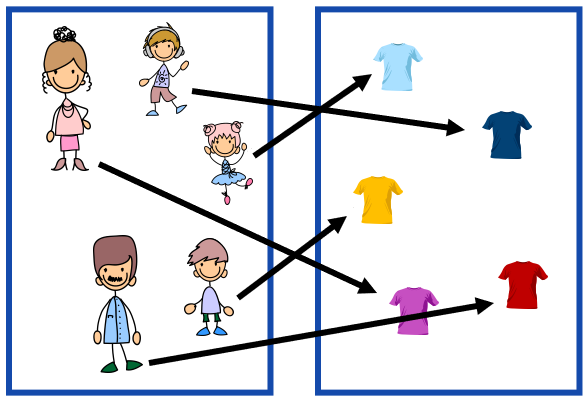
\includegraphics{pics/c_3.png}
\end{image}
\end{center}




\textbf{Pants}

\begin{center}
(arrows go from the domain to the codomain.)
\begin{image}
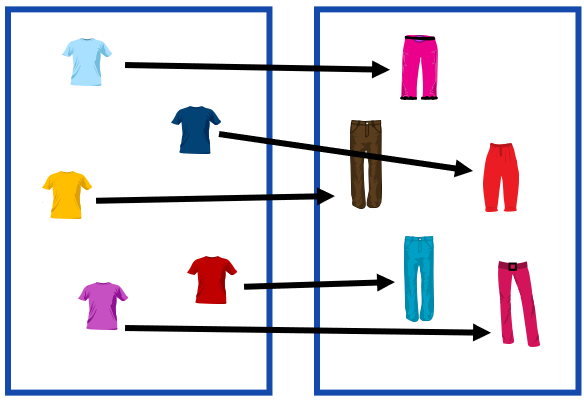
\includegraphics{pics/c_6.png}
\end{image}
\end{center}



Now define a new function called \textbf{Dressing}.


\begin{center}
\textbf{$Dressing = Pants \circ Shirts$}
\end{center}

\begin{center}
$Dressing$(
\includegraphics{pics/0.png}) = ($Pants \circ Shirts$)(
\includegraphics{pics/0.png}))
\end{center}

\begin{center}
$Dressing$(
\includegraphics{pics/0.png}) = $Pants$($Shirts$(
\includegraphics{pics/0.png}))
\end{center}

\begin{center}
= $Pants$(
\includegraphics{pics/10.png})
\end{center}

\begin{center}
= 
\includegraphics{pics/20.png}
\end{center}



\end{example}

Everything has to fit together for a composition to work.


The domain of $Dressing$ is a subset of the domain of $Shirts$.  

The range of $Dressing$ is a subset of the range of $Pants$.














\begin{example} Composition

Let $Outfit$ and $Person$ be the two functions represented by the maps below.

\textbf{Outfit}

\begin{center}
(arrows go from the domain to the codomain.)
\begin{image}
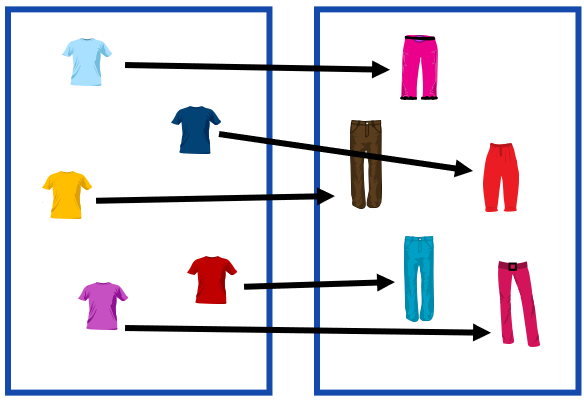
\includegraphics{pics/c_6.png}
\end{image}
\end{center}




\textbf{Person}

\begin{center}
(arrows go from the domain to the codomain.)
\begin{image}
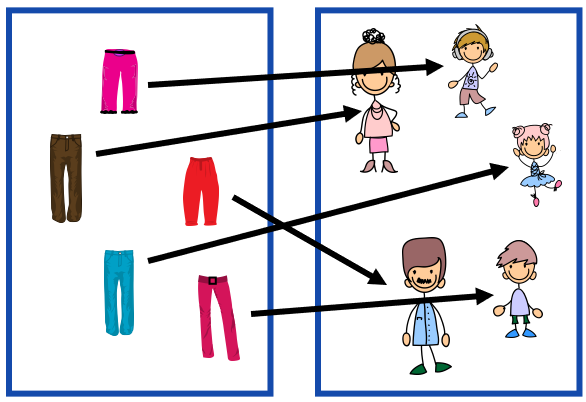
\includegraphics{pics/c_1.png}
\end{image}
\end{center}



Now define a new function called \textbf{Dressed}.


\begin{center}
\textbf{$Dressed = Person \circ Outfit$}
\end{center}

\begin{center}
$Dressed$(
\includegraphics{pics/9.png}) = ($Person \circ Outfit$)(
\includegraphics{pics/9.png})
\end{center}

\begin{center}
$Dressed$(
\includegraphics{pics/9.png}) = $Person$($Outfit$(
\includegraphics{pics/9.png}))
\end{center}

\begin{center}
= $Person$(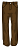
\includegraphics{pics/17.png})
\end{center}

\begin{center}
= 
\includegraphics{pics/0.png}
\end{center}



\end{example}


\textbf{Note:} In the previous example, we could not form the composition $Outfit \circ Person$, because the values of the function $Person$ are not members of the domain of the function $Outfit$.








\subsection*{A New Function}

The composition of two functions is a new function. It links together two existing functions together to form a brand new function.

\begin{itemize}
\item The domain of the composition is a subset of the domain of the first (inner) function.
\item The range of the composition is a subset of the range of the second (outer) function.
\end{itemize}

To evaluate the composition, you make a pitstop in between the domain of the composition and the range of the composition.

\begin{center}
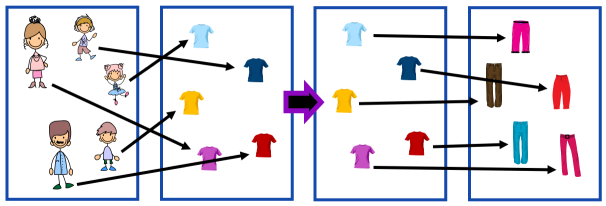
\includegraphics{pics/comp_chain_1sm.png}
\end{center}

But, really, you can ignore the pistop and just think of the composition as its own function.


\begin{center}
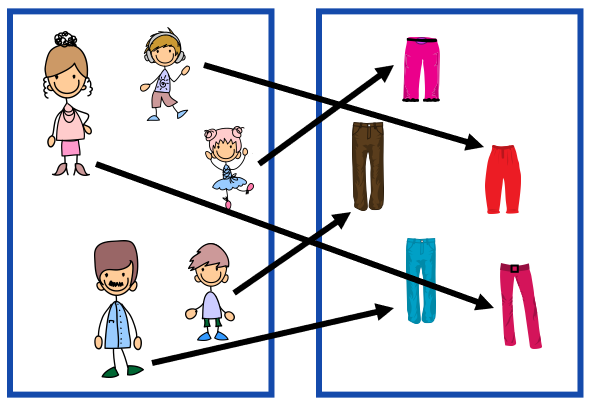
\includegraphics{pics/comp_full_1.png}
\end{center}




We are chaining two functions together, which means they must match up.

\begin{center}

\textbf{The range of the inner function has to be inside the domain of the outer function.}

If they don't match up, then we must adjust the domain of the outer function.

\end{center}





\begin{explanation} \textbf{\textcolor{red!75!green}{Matching}} 

Consider this situation:

We have two functions: $Inner$ and $Outer$.

We want to form the composition: $Outer \circ Inner$.

Suppose $A$ is in the domain of $Inner$, but $Inner(A)$ is not a member of the domain of $Outer$.

In this case, we need to remove $A$ from the domain of the composition.




\end{explanation}











\begin{example} Composition


Let $Inner$ and $Outer$ be the two functions represented by the maps below.

\textbf{Inner}

\begin{center}
(arrows go from the domain to the codomain.)
\begin{image}
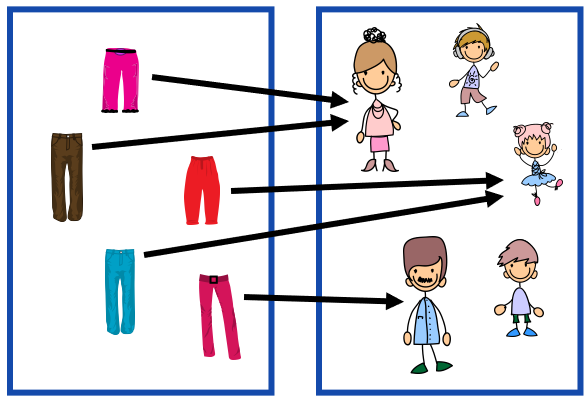
\includegraphics{pics/c_7.png}
\end{image}
\end{center}




\textbf{Outer}

\begin{center}
(arrows go from the domain to the codomain.)
\begin{image}
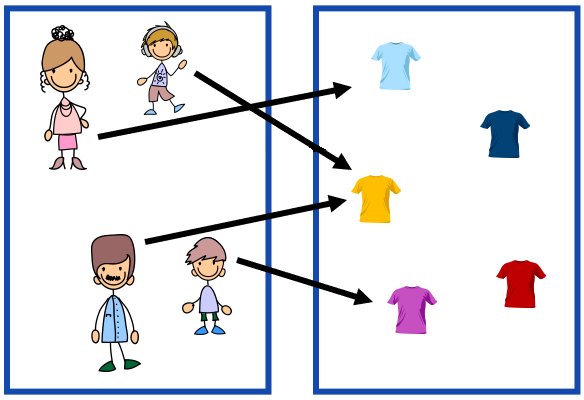
\includegraphics{pics/c_9.png}
\end{image}
\end{center}



Notice that $Inner($
\includegraphics{pics/18.png})$ = $
\includegraphics{pics/2.png}

And, 
\includegraphics{pics/2.png} is not in the domain of $Outer$.


Therefore, 
\includegraphics{pics/18.png} cannot be in the domain of the composition.



Keeping this in mind, let's define the composition function, which is a new function called \textbf{C}.


\begin{center}
\textbf{$C = Outer \circ Inner$}
\end{center}


We must modify the domain.



\begin{center}
(arrows go from the domain to the codomain.)
\begin{image}
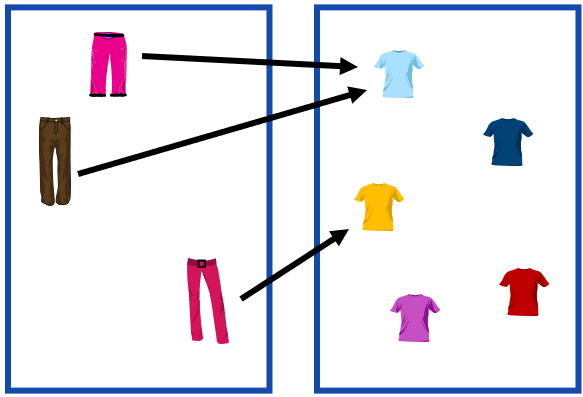
\includegraphics{pics/comp_full_2.png}
\end{image}
\end{center}




We had to remove both 
\includegraphics{pics/18.png} and 
\includegraphics{pics/19.png}, because they both had 
\includegraphics{pics/2.png} as their image in the $Inner$ function.



\end{example}




This is very common.

This type of domain and range modification for compositions happens all of the time.

We will encounter this kind of activity every time we look at compositions, which is all the time.


















\begin{example} Composition







Let $P$ and $M$ be the two functions represented by the maps below.

\textbf{M}

\begin{center}
(arrows go from the domain to the codomain.)
\begin{image}
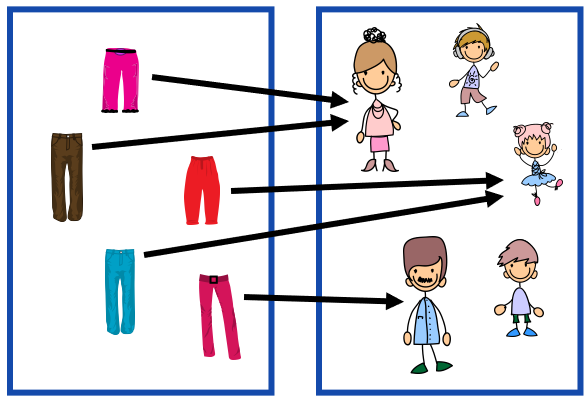
\includegraphics{pics/c_7.png}
\end{image}
\end{center}




\textbf{P}

\begin{center}
(arrows go from the domain to the codomain.)
\begin{image}
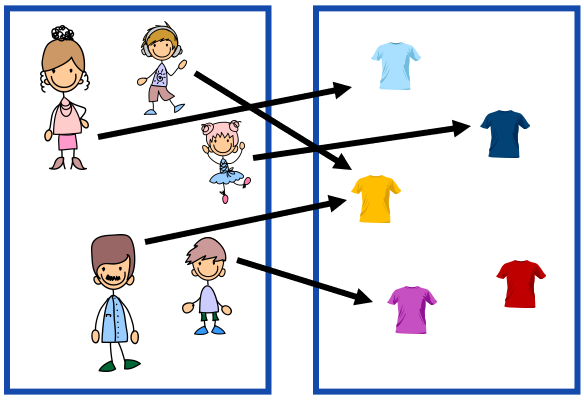
\includegraphics{pics/c_8.png}
\end{image}
\end{center}


Now define $B = P \circ M$ as the composition function.



\begin{question}


What is the image of 
\includegraphics{../../pics/func_maps/pieces/16.png} under the $B$ function?

\begin{multipleChoice}
\choice {
\includegraphics{../../pics/func_maps/pieces/2.png}}
\choice [correct]{
\includegraphics{../../pics/func_maps/pieces/19.png}}
\choice {
\includegraphics{../../pics/func_maps/pieces/6.png}}
\choice {
\includegraphics{../../pics/func_maps/pieces/9.png}}
\choice {
\includegraphics{../../pics/func_maps/pieces/10.png}}
\choice {
\includegraphics{../../pics/func_maps/pieces/7.png}}
\choice {
\includegraphics{../../pics/func_maps/pieces/8.png}}
\choice {No Value}
\end{multipleChoice}

\end{question}







\begin{question}


Evaluate $B($
\includegraphics{../../pics/func_maps/pieces/19.png}$)$. 


\begin{multipleChoice}
\choice {
\includegraphics{../../pics/func_maps/pieces/2.png}}
\choice {
\includegraphics{../../pics/func_maps/pieces/19.png}}
\choice {
\includegraphics{../../pics/func_maps/pieces/6.png}}
\choice {
\includegraphics{../../pics/func_maps/pieces/9.png}}
\choice {
\includegraphics{../../pics/func_maps/pieces/10.png}}
\choice [correct]{
\includegraphics{../../pics/func_maps/pieces/7.png}}
\choice {
\includegraphics{../../pics/func_maps/pieces/8.png}}
\choice {No Value}
\end{multipleChoice}

\end{question}










\begin{question}


Select all items of the range of $B$. 


\begin{selectAll}
\choice [correct]{
\includegraphics{../../pics/func_maps/pieces/6.png}}
\choice [correct]{
\includegraphics{../../pics/func_maps/pieces/9.png}}
\choice {
\includegraphics{../../pics/func_maps/pieces/10.png}}
\choice [correct]{
\includegraphics{../../pics/func_maps/pieces/7.png}}
\choice {
\includegraphics{../../pics/func_maps/pieces/8.png}}
\choice {No Value}
\end{selectAll}

\end{question}




\end{example}






\subsection*{Chaining}


We can chain together any number of functions as long as their domains and ranges match.



\textbf{For Instance,} the functions $F$, $G$, and $H$ are defined as follows.



\textbf{F:} \\
domain: $\{ 1, 2, 3 \}$ \\
range: $\{ 4, 5, 6 \}$ \\
pairs: $\{ (1, 4), (2, 5) , (3, 6) \}$ \\


\textbf{G:} \\
domain: $\{ 4, 5, 6 \}$ \\
range: $\{ A, B, C \}$ \\
pairs: $\{ (4, A), (5, B), (6, C) \}$ \\



\textbf{H:} \\
domain: $\{ A, B, C \}$ \\
range: $\{ 9, 8, 7 \}$ \\
pairs: $\{ (A, 9), (B, 8), (C, 7) \}$ \\



Then, we could define a new function, $M$, as a composition.

\[ M = H \circ G \circ F \]



\textbf{M:} \\
domain: $\{ 1, 2, 3 \}$ \\
range: $\{ 9, 8, 7 \}$ \\
pairs: $\{ (1, 9), (2, 8) , (3, 7) \}$ \\


Each pair in $M$ required gluing together three pairs.


\[ (1, 9) = (1,4) \bigoplus (4, A) \bigoplus (A, 9) \]











\begin{onlineOnly}
\begin{center}
\textbf{\textcolor{green!50!black}{ooooo-=-=-=-ooOoo-=-=-=-ooooo}} \\

more examples can be found by following this link\\ \link[More Examples of Functions]{https://ximera.osu.edu/csccmathematics/precalculus/precalculus/functions/examples/exampleList}

\end{center}
\end{onlineOnly}





\end{document}
